\chapter{Tutorial}\label{chap:tutorial}
This chapter explains how to start \Pink and how to use it.

\section{Starting \Pink and related software}


\section{Examples}

We will show a lot of Python code:
\subsection{Code highlighting}
Testing Listings:
\lstinputlisting{python/tut/hello.py}

Testing fancyvrb
\lstset{language=Python}

\pylabel{prog1}
\VerbatimInput[label=\fbox{\textbf{Program \ref{prog1}:} hello in Python}]{"python/tut/hello.py"}




\subsection{Dynamic content}
%% some embedded python
\begin{figure}
\centering
\begin{python}
import sys
sys.path.append('python/test')
import matplotlib
# non-interactive backend
matplotlib.use('PDF') 
##
import plottest01
##
matplotlib.pyplot.savefig('dynamic/multiaxis.pdf')
print r'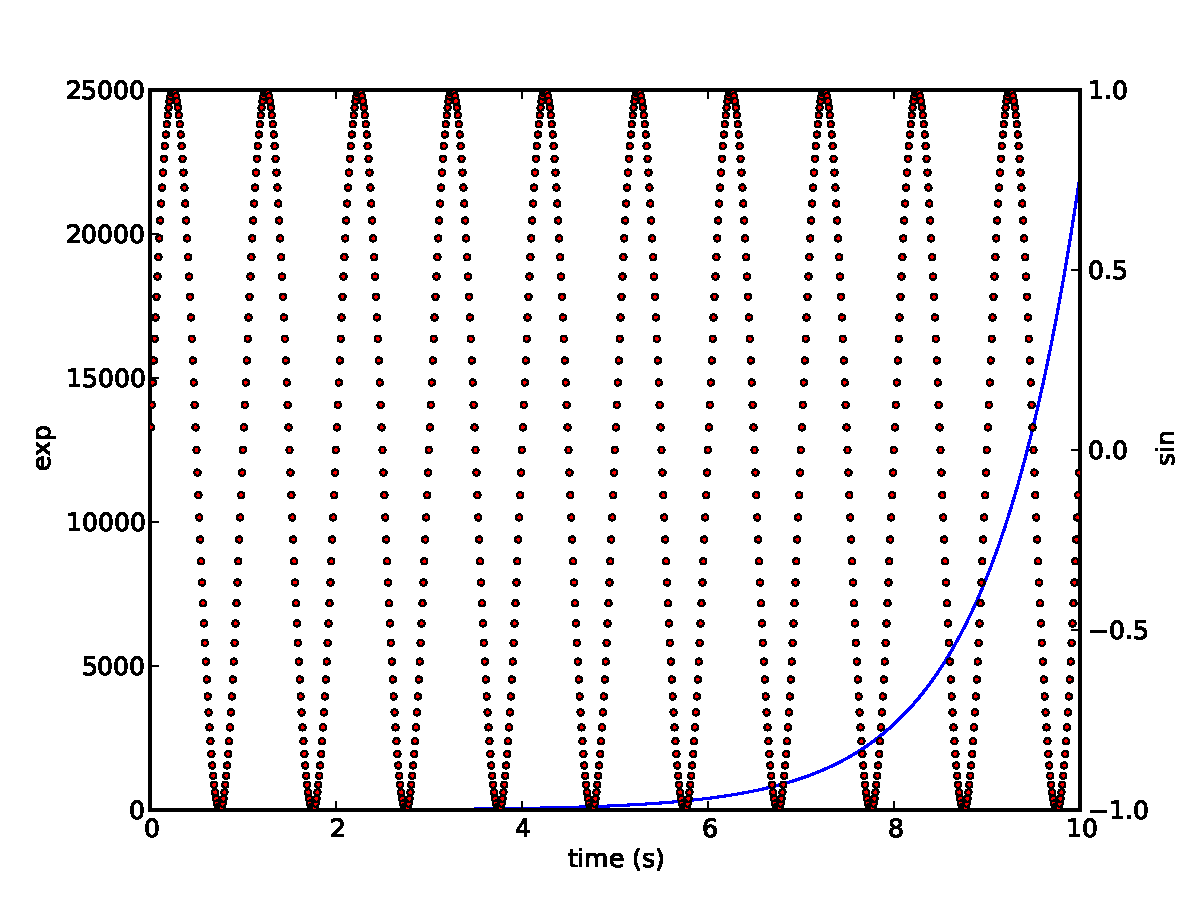
\includegraphics[width=0.5\textwidth]{dynamic/multiaxis.pdf}'
\end{python}
\caption{The functions $\sin$ and $\exp$ together from program~\ref{prog2}.\label{fig:plot2}}
\end{figure}

Some code and its output: The following program produces the plot from Fig.~\ref{fig:plot2}.

\pylabel{prog2}
\VerbatimInput[label=\fbox{\textbf{Program \ref{prog2}:} A plotting example}]{"python/test/plottest01.py"}

\subsection{Image processing}
An example of processing?

\begin{figure}
\centering
\begin{python}
import sys
sys.path.append('python/test')
import matplotlib
import numpy as np
# non-interactive backend
matplotlib.use('PDF') 
## real work done here

import plottest02

## plotting done here
plottest02.saveimages('dynamic/sampleinput.pdf', 'dynamic/sampleoutput.pdf')
## result
print r'\subfigure[]{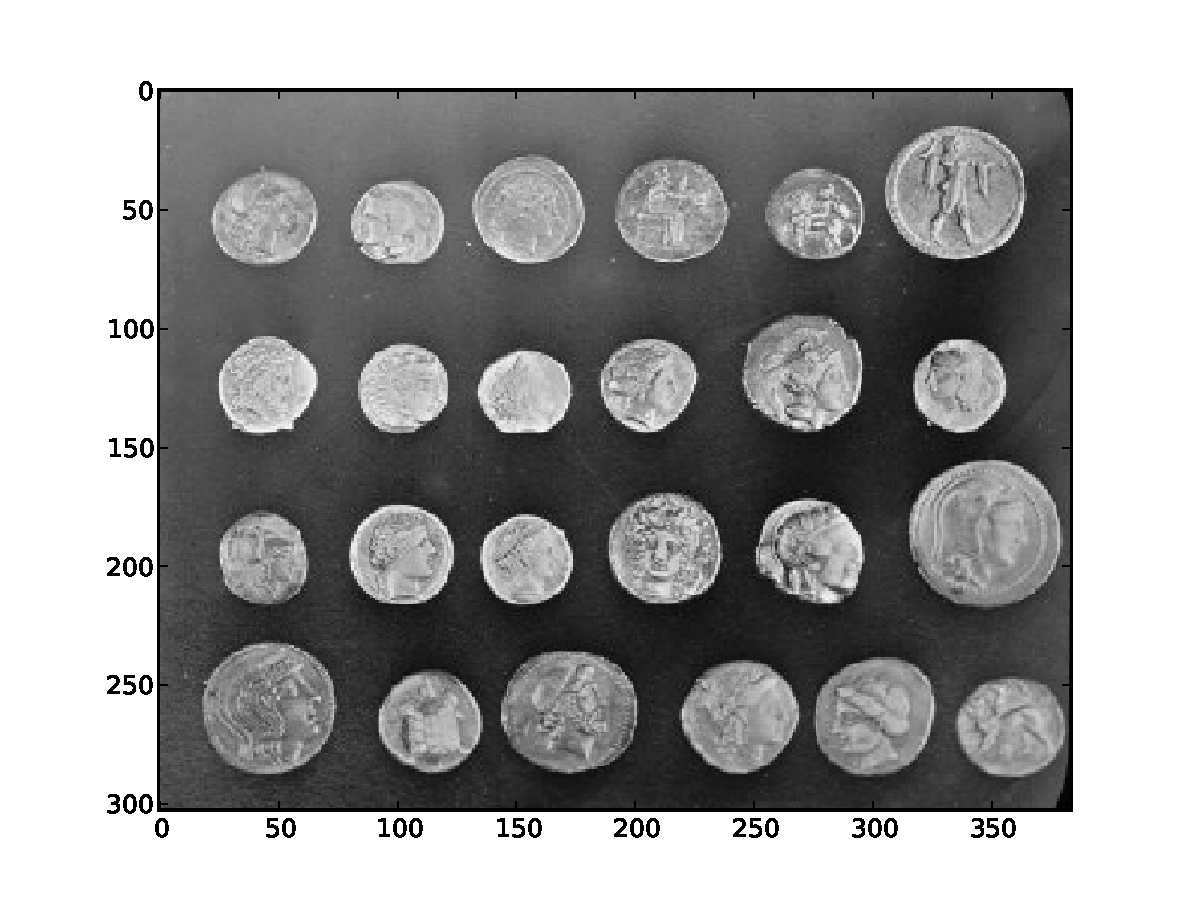
\includegraphics[width=0.45\textwidth]{dynamic/sampleinput.pdf}}'
print r'\subfigure[]{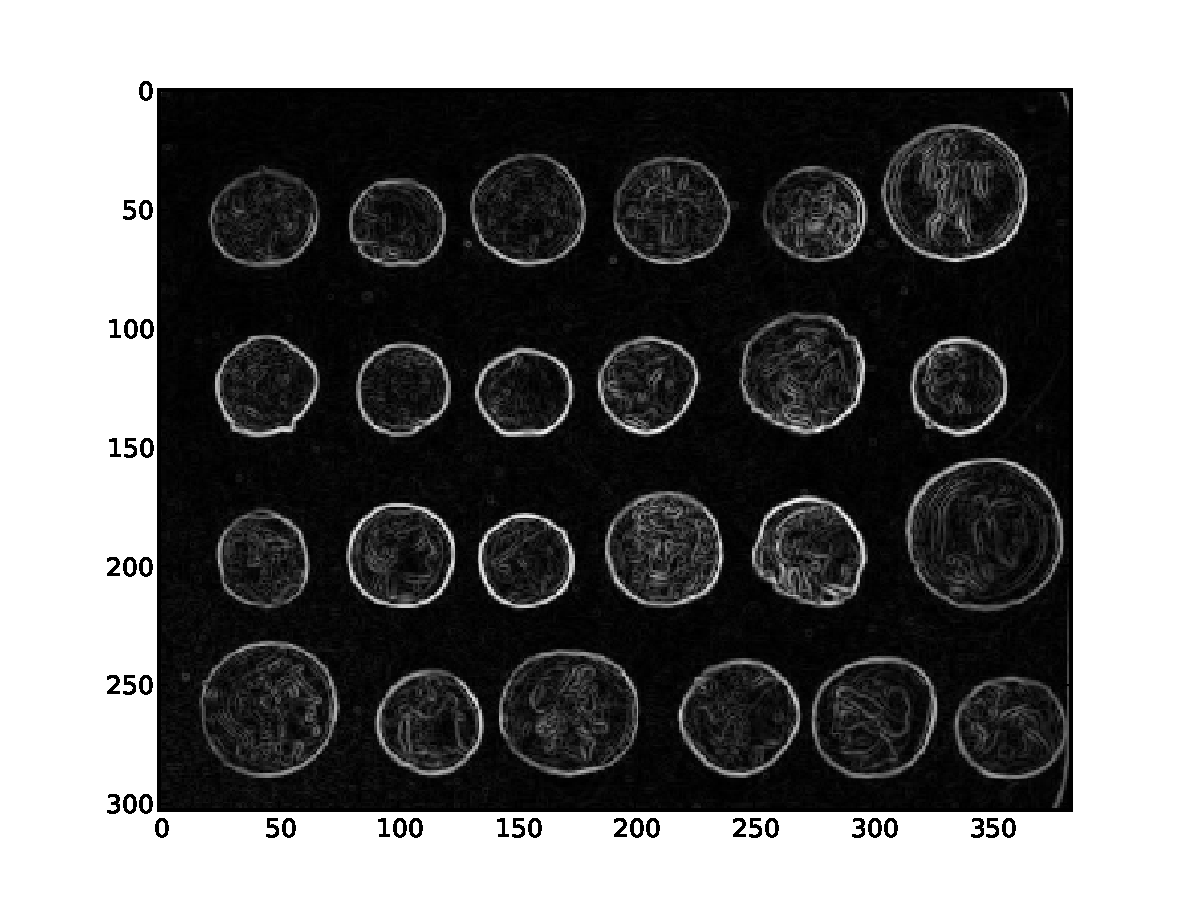
\includegraphics[width=0.45\textwidth]{dynamic/sampleoutput.pdf}}'
\end{python}
\pylabel{prog3}
\VerbatimInput[firstline=2,lastline=13,label=\fbox{\textbf{Program \ref{prog3}:} An image processing example}]{"python/test/plottest02.py"}
\caption{Program~\ref{prog3} and its result.}
\end{figure}





\subsection{Binary image processing}

\subsection{Grey-level segmentation}

\subsection{Discrete geometry}

\subsection{3D image processing}

\section{\Pink and other image-related software}

\subsection{\Pink and numpy}

\subsection{\Pink and scikit}

\subsection{\Pink and VTK}

\subsection{\Pink and ITK}

\section{Exercises}

